% Options for packages loaded elsewhere
\PassOptionsToPackage{unicode}{hyperref}
\PassOptionsToPackage{hyphens}{url}
\PassOptionsToPackage{dvipsnames,svgnames,x11names}{xcolor}
%
\documentclass[
  letterpaper,
  DIV=11,
  numbers=noendperiod]{scrreprt}

\usepackage{amsmath,amssymb}
\usepackage{lmodern}
\usepackage{iftex}
\ifPDFTeX
  \usepackage[T1]{fontenc}
  \usepackage[utf8]{inputenc}
  \usepackage{textcomp} % provide euro and other symbols
\else % if luatex or xetex
  \usepackage{unicode-math}
  \defaultfontfeatures{Scale=MatchLowercase}
  \defaultfontfeatures[\rmfamily]{Ligatures=TeX,Scale=1}
\fi
% Use upquote if available, for straight quotes in verbatim environments
\IfFileExists{upquote.sty}{\usepackage{upquote}}{}
\IfFileExists{microtype.sty}{% use microtype if available
  \usepackage[]{microtype}
  \UseMicrotypeSet[protrusion]{basicmath} % disable protrusion for tt fonts
}{}
\makeatletter
\@ifundefined{KOMAClassName}{% if non-KOMA class
  \IfFileExists{parskip.sty}{%
    \usepackage{parskip}
  }{% else
    \setlength{\parindent}{0pt}
    \setlength{\parskip}{6pt plus 2pt minus 1pt}}
}{% if KOMA class
  \KOMAoptions{parskip=half}}
\makeatother
\usepackage{xcolor}
\setlength{\emergencystretch}{3em} % prevent overfull lines
\setcounter{secnumdepth}{5}
% Make \paragraph and \subparagraph free-standing
\ifx\paragraph\undefined\else
  \let\oldparagraph\paragraph
  \renewcommand{\paragraph}[1]{\oldparagraph{#1}\mbox{}}
\fi
\ifx\subparagraph\undefined\else
  \let\oldsubparagraph\subparagraph
  \renewcommand{\subparagraph}[1]{\oldsubparagraph{#1}\mbox{}}
\fi


\providecommand{\tightlist}{%
  \setlength{\itemsep}{0pt}\setlength{\parskip}{0pt}}\usepackage{longtable,booktabs,array}
\usepackage{calc} % for calculating minipage widths
% Correct order of tables after \paragraph or \subparagraph
\usepackage{etoolbox}
\makeatletter
\patchcmd\longtable{\par}{\if@noskipsec\mbox{}\fi\par}{}{}
\makeatother
% Allow footnotes in longtable head/foot
\IfFileExists{footnotehyper.sty}{\usepackage{footnotehyper}}{\usepackage{footnote}}
\makesavenoteenv{longtable}
\usepackage{graphicx}
\makeatletter
\def\maxwidth{\ifdim\Gin@nat@width>\linewidth\linewidth\else\Gin@nat@width\fi}
\def\maxheight{\ifdim\Gin@nat@height>\textheight\textheight\else\Gin@nat@height\fi}
\makeatother
% Scale images if necessary, so that they will not overflow the page
% margins by default, and it is still possible to overwrite the defaults
% using explicit options in \includegraphics[width, height, ...]{}
\setkeys{Gin}{width=\maxwidth,height=\maxheight,keepaspectratio}
% Set default figure placement to htbp
\makeatletter
\def\fps@figure{htbp}
\makeatother
\newlength{\cslhangindent}
\setlength{\cslhangindent}{1.5em}
\newlength{\csllabelwidth}
\setlength{\csllabelwidth}{3em}
\newlength{\cslentryspacingunit} % times entry-spacing
\setlength{\cslentryspacingunit}{\parskip}
\newenvironment{CSLReferences}[2] % #1 hanging-ident, #2 entry spacing
 {% don't indent paragraphs
  \setlength{\parindent}{0pt}
  % turn on hanging indent if param 1 is 1
  \ifodd #1
  \let\oldpar\par
  \def\par{\hangindent=\cslhangindent\oldpar}
  \fi
  % set entry spacing
  \setlength{\parskip}{#2\cslentryspacingunit}
 }%
 {}
\usepackage{calc}
\newcommand{\CSLBlock}[1]{#1\hfill\break}
\newcommand{\CSLLeftMargin}[1]{\parbox[t]{\csllabelwidth}{#1}}
\newcommand{\CSLRightInline}[1]{\parbox[t]{\linewidth - \csllabelwidth}{#1}\break}
\newcommand{\CSLIndent}[1]{\hspace{\cslhangindent}#1}

\KOMAoption{captions}{tableheading}
\makeatletter
\@ifpackageloaded{tcolorbox}{}{\usepackage[many]{tcolorbox}}
\@ifpackageloaded{fontawesome5}{}{\usepackage{fontawesome5}}
\definecolor{quarto-callout-color}{HTML}{909090}
\definecolor{quarto-callout-note-color}{HTML}{0758E5}
\definecolor{quarto-callout-important-color}{HTML}{CC1914}
\definecolor{quarto-callout-warning-color}{HTML}{EB9113}
\definecolor{quarto-callout-tip-color}{HTML}{00A047}
\definecolor{quarto-callout-caution-color}{HTML}{FC5300}
\definecolor{quarto-callout-color-frame}{HTML}{acacac}
\definecolor{quarto-callout-note-color-frame}{HTML}{4582ec}
\definecolor{quarto-callout-important-color-frame}{HTML}{d9534f}
\definecolor{quarto-callout-warning-color-frame}{HTML}{f0ad4e}
\definecolor{quarto-callout-tip-color-frame}{HTML}{02b875}
\definecolor{quarto-callout-caution-color-frame}{HTML}{fd7e14}
\makeatother
\makeatletter
\makeatother
\makeatletter
\@ifpackageloaded{bookmark}{}{\usepackage{bookmark}}
\makeatother
\makeatletter
\@ifpackageloaded{caption}{}{\usepackage{caption}}
\AtBeginDocument{%
\ifdefined\contentsname
  \renewcommand*\contentsname{Table of contents}
\else
  \newcommand\contentsname{Table of contents}
\fi
\ifdefined\listfigurename
  \renewcommand*\listfigurename{List of Figures}
\else
  \newcommand\listfigurename{List of Figures}
\fi
\ifdefined\listtablename
  \renewcommand*\listtablename{List of Tables}
\else
  \newcommand\listtablename{List of Tables}
\fi
\ifdefined\figurename
  \renewcommand*\figurename{Figure}
\else
  \newcommand\figurename{Figure}
\fi
\ifdefined\tablename
  \renewcommand*\tablename{Table}
\else
  \newcommand\tablename{Table}
\fi
}
\@ifpackageloaded{float}{}{\usepackage{float}}
\floatstyle{ruled}
\@ifundefined{c@chapter}{\newfloat{codelisting}{h}{lop}}{\newfloat{codelisting}{h}{lop}[chapter]}
\floatname{codelisting}{Listing}
\newcommand*\listoflistings{\listof{codelisting}{List of Listings}}
\makeatother
\makeatletter
\@ifpackageloaded{caption}{}{\usepackage{caption}}
\@ifpackageloaded{subcaption}{}{\usepackage{subcaption}}
\makeatother
\makeatletter
\@ifpackageloaded{tcolorbox}{}{\usepackage[many]{tcolorbox}}
\makeatother
\makeatletter
\@ifundefined{shadecolor}{\definecolor{shadecolor}{rgb}{.97, .97, .97}}
\makeatother
\makeatletter
\makeatother
\ifLuaTeX
  \usepackage{selnolig}  % disable illegal ligatures
\fi
\IfFileExists{bookmark.sty}{\usepackage{bookmark}}{\usepackage{hyperref}}
\IfFileExists{xurl.sty}{\usepackage{xurl}}{} % add URL line breaks if available
\urlstyle{same} % disable monospaced font for URLs
\hypersetup{
  pdftitle={Palmyra Atoll Data Library},
  colorlinks=true,
  linkcolor={blue},
  filecolor={Maroon},
  citecolor={Blue},
  urlcolor={Blue},
  pdfcreator={LaTeX via pandoc}}

\title{Palmyra Atoll Data Library}
\author{}
\date{}

\begin{document}
\maketitle
\ifdefined\Shaded\renewenvironment{Shaded}{\begin{tcolorbox}[breakable, sharp corners, interior hidden, boxrule=0pt, borderline west={3pt}{0pt}{shadecolor}, enhanced, frame hidden]}{\end{tcolorbox}}\fi

\renewcommand*\contentsname{Table of contents}
{
\hypersetup{linkcolor=}
\setcounter{tocdepth}{2}
\tableofcontents
}
\bookmarksetup{startatroot}

\hypertarget{welcome}{%
\chapter*{Welcome!}\label{welcome}}
\addcontentsline{toc}{chapter}{Welcome!}

The Palmyra Atoll Data Library (PADL) aims to publish as much data
collected at Palmyra Atoll as possible.

We believe that facilitating access to research and its associated data
will amplify academic discussions, help other researchers, and further
inform management and policy decisions being made in Palmyra and other
tropical ecosystems.

We are working with the \href{https://edirepository.org/}{Environmental
Data Initiative (EDI)}, an NSF-supported initiative that provides a
reliable, registered and certified trustworthy data repository with an
open-access API. EDI follows a high metadata standard that ensures that
your future self and others can utilize data for scientific and other
forms of inquiry.

\hypertarget{why-padl}{%
\subsection*{Why PADL?}\label{why-padl}}
\addcontentsline{toc}{subsection}{Why PADL?}

We want to have a centralized place where scientist and managers have
access to all data collected at Palmyra Atoll. We believe that data are
among the most valuable outputs of research. If no-one can access these
data, all the data collection is a shocking waste of resources. Having
an open data library allows for aggregating and synthesizing data from
different contexts. This is essential to establishing broader ecological
knowledge and informing conservation management. Long-term data are
crucial to understand historical patterns and baselines in a changing
world. PADL wants to make it easy for scientist to know and have access
to research done at Palmyra in the past.

\begin{tcolorbox}[enhanced jigsaw, colbacktitle=quarto-callout-note-color!10!white, title=\textcolor{quarto-callout-note-color}{\faInfo}\hspace{0.5em}{Note}, colframe=quarto-callout-note-color-frame, arc=.35mm, rightrule=.15mm, colback=white, toptitle=1mm, titlerule=0mm, toprule=.15mm, bottomtitle=1mm, bottomrule=.15mm, leftrule=.75mm, opacityback=0, breakable, coltitle=black, opacitybacktitle=0.6, left=2mm]
This guide borrows heavily from
\href{https://edirepository.org/resources/resources-for-data-authors}{EDI
resources},
\href{https://caplter.github.io/caplter_ezeml/\#getting-started}{CAP
LTER Getting Started Guide} and
\href{https://www.nceas.ucsb.edu/learning-hub/core-r}{NCEAS coreR
curriculum}. Check out the links and see complete citation on the
reference section.
\end{tcolorbox}

\bookmarksetup{startatroot}

\hypertarget{about-this-guide}{%
\chapter*{About this guide}\label{about-this-guide}}
\addcontentsline{toc}{chapter}{About this guide}

We created this guide to help you document your data in a way that
facilitates the process of publishing your data or metadata to EDI. Here
we describe what you need to do to make your data publicly available
through the EDI repository.

\begin{tcolorbox}[enhanced jigsaw, colbacktitle=quarto-callout-important-color!10!white, title=\textcolor{quarto-callout-important-color}{\faExclamation}\hspace{0.5em}{Important}, colframe=quarto-callout-important-color-frame, arc=.35mm, rightrule=.15mm, colback=white, toptitle=1mm, titlerule=0mm, toprule=.15mm, bottomtitle=1mm, bottomrule=.15mm, leftrule=.75mm, opacityback=0, breakable, coltitle=black, opacitybacktitle=0.6, left=2mm]
We understand that EDI might not be suitable to all data. If you are
planning to publish you data elsewhere we ask to please collect the
metadata following EDI metadata standards presented in this guide and
submit your metadata to TNC Palmyra.
\end{tcolorbox}

\hypertarget{what-to-expect}{%
\subsection*{What to expect}\label{what-to-expect}}
\addcontentsline{toc}{subsection}{What to expect}

\begin{itemize}
\tightlist
\item
  The goal of this guide is for you to know what you need to do to be in
  compliance with TNC Palmyra Data Sharing Agreement.
\item
  We provide some orientation and tips for when planning your data
  collection, together with resources to learn more about tidy data.
\item
  We describe each of the elements needed to best document your data.
\item
  This guide goes in-depth on how to publish your data using the
  \href{https://ezeml.edirepository.org/eml/}{ezEML} tool suite
  developed by the Environmental Data Initiative
  \href{https://edirepository.org/}{(EDI)}.
\item
  We also provide metadata templates for you to know and plan on
  documenting your data from the get go.
\end{itemize}

\begin{tcolorbox}[enhanced jigsaw, colbacktitle=quarto-callout-color!10!white, title={Recommendation}, colframe=quarto-callout-color-frame, arc=.35mm, rightrule=.15mm, colback=white, toptitle=1mm, titlerule=0mm, toprule=.15mm, bottomtitle=1mm, bottomrule=.15mm, leftrule=.75mm, opacityback=0, breakable, coltitle=black, opacitybacktitle=0.6, left=2mm]
We highly recommend to have a plan for collecting your metadata since
the beginning of your research life cycle. According to EDI experience
``continuous creation of metadata during the research life cycle greatly
benefits data management during a project and when it comes time to
publish data when the project concludes''.
\end{tcolorbox}

\begin{figure}

{\centering 

\href{https://edirepository.org/resources/creating-metadata-during-the-research-lifecycle}{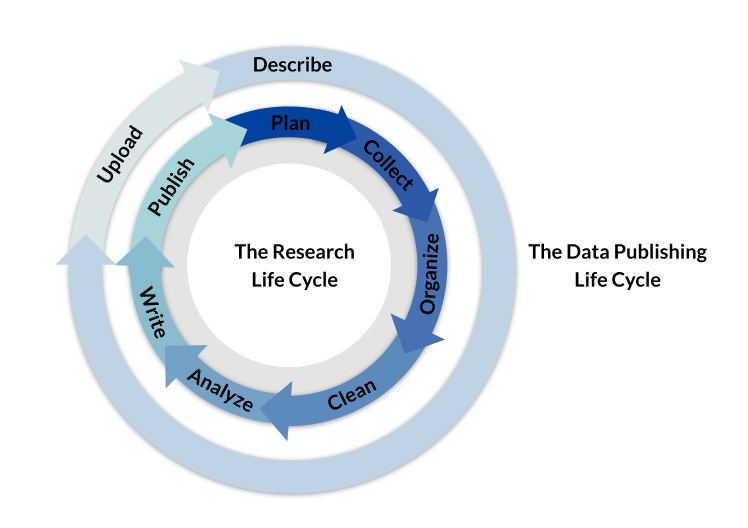
\includegraphics{content/pics/metadata-in-the-research-life-cycle.png}}

}

\caption{from edirepository.org, Creating Metadata During the Research
Life Cycle}

\end{figure}

\bookmarksetup{startatroot}

\hypertarget{basic-concepts}{%
\chapter*{Basic Concepts}\label{basic-concepts}}
\addcontentsline{toc}{chapter}{Basic Concepts}

Before we start we want to introduce to some relevant concepts related
to data publishing. This sets the ground to navigate the
environmental/ecological data publishing world.

\textbf{Data Package}

\begin{itemize}
\item
  EDI publishes data from the ecological and environmental sciences
  irrespective of funding origin.
\item
  The \emph{unit of publication} is called a data package.
\item
  This is an assemblage of science metadata, the data it self, and any
  other file you want to publish with your data.
\item
  The basic rule of thumb is to package your data in the form you would
  like to receive it.
\item
  Each data package is assigned a Digital Object Identifier (DOI) and
  published in the repository for future use.
\item
  EDI resources on
  \href{https://edirepository.org/resources/the-data-package}{data
  packages}
\end{itemize}

\textbf{Metadata}

\begin{itemize}
\tightlist
\item
  The metadata is the data that provides information about your data. It
  describe the structure, content, and context of your data.
\item
  They are vital to the discovery and reuse of data, and are a required
  element of a data package.
\item
  EDI resources on
  \href{https://edirepository.org/resources/creating-metadata-for-publication}{Creating
  Metadata for a Data Package}
\end{itemize}

\textbf{Ecological Metadata Language (EML)}

\begin{itemize}
\tightlist
\item
  EDI uses the Ecological Metadata Language (EML) format to document the
  metadata in each data package.
\item
  ``EML provides a comprehensive vocabulary and a readable XML markup
  syntax for documenting research data. It is a community-maintained
  specification, and evolves to meet the data documentation needs of
  researchers who want to openly document, preserve, and share data and
  outputs'' (\href{https://eml.ecoinformatics.org/}{Jones et al, 2019}).
\end{itemize}

\textbf{ezEML}

\begin{itemize}
\item
  EDI created a user-friendly tool that streamlined the process of the
  creating metadata in the Ecological Metadata Language (EML).
\item
  ezEML is a form-based online application that leads the user through
  EML document creation step by step.
\item
  Check out EDI
  \href{https://ezeml.edirepository.org/eml/user_guide}{ezEML User
  Guide} for more information.
\end{itemize}

\bookmarksetup{startatroot}

\hypertarget{data-workflow}{%
\chapter{Data Workflow}\label{data-workflow}}

\begin{enumerate}
\def\labelenumi{\arabic{enumi}.}
\tightlist
\item
  Organize
\item
  Clean
\item
  Describe
\item
  Upload
\item
  Cite
\end{enumerate}

\bookmarksetup{startatroot}

\hypertarget{metadata-describing-your-data-in-eml}{%
\chapter{Metadata: Describing your data in
EML}\label{metadata-describing-your-data-in-eml}}

This section presents a description of the most relevat components of
EML. The goal is for you to familiarize with all that you need to
document from your data. The next sections show different ways for you
to do this allong the way.

\bookmarksetup{startatroot}

\hypertarget{set-up}{%
\chapter*{Set Up}\label{set-up}}
\addcontentsline{toc}{chapter}{Set Up}

\bookmarksetup{startatroot}

\hypertarget{references}{%
\chapter*{References}\label{references}}
\addcontentsline{toc}{chapter}{References}

\hypertarget{refs}{}
\begin{CSLReferences}{0}{0}
\end{CSLReferences}

\bookmarksetup{startatroot}

\hypertarget{other-options-for-creating-emls}{%
\chapter*{Other options for creating
EMLs''}\label{other-options-for-creating-emls}}
\addcontentsline{toc}{chapter}{Other options for creating EMLs''}

\bookmarksetup{startatroot}

\hypertarget{additional-resources}{%
\chapter*{Additional Resources}\label{additional-resources}}
\addcontentsline{toc}{chapter}{Additional Resources}



\end{document}
